\documentclass[sigconf]{acmart}

\usepackage{color}
\usepackage{graphicx}
\usepackage{url}
\usepackage{balance}

% \usepackage{draftwatermark}\SetWatermarkFontSize{4cm}\SetWatermarkText{DRAFT v4.29}


%----------

\AtBeginDocument{%
  \providecommand\BibTeX{{%
    \normalfont B\kern-0.5em{\scshape i\kern-0.25em b}\kern-0.8em\TeX}}}

%% Rights management information.  This information is sent to you
%% when you complete the rights form.  These commands have SAMPLE
%% values in them; it is your responsibility as an author to replace
%% the commands and values with those provided to you when you
%% complete the rights form.
\copyrightyear{2026}
\acmYear{2026}
\setcopyright{cc}
\setcctype{by}
\acmConference[SIGCSE Virtual 2026] {Proceedings of the 2nd ACM Virtual Global Computing Education Conference V.1}{November 12--15, 2026}{Virtual Event, USA.}
\acmBooktitle{Proceedings of the 2nd ACM Virtual Global Computing Education Conference V.1 (SIGCSE Virtual 2026), November 12--15, 2026, Virtual Event, USA}
\acmISBN{979-8-4007-2506-7/2026/11}
\acmDOI{10.1145/3795867.3830974}
% 1 Authors, replace the red X's with your assigned DOI string during the rightsreview eform process.
% 2 Your DOI link will become active when the proceedings appears in the DL.
% 3 Retain the DOI string between the curly braces for uploading your promo video.

\settopmatter{printacmref=true}

%%
%% Submission ID.
%% Use this when submitting an article to a sponsored event. You'll
%% receive a unique submission ID from the organizers
%% of the event, and this ID should be used as the parameter to this command.
%%\acmSubmissionID{123-A56-BU3}

%%
%% For managing citations, it is recommended to use bibliography
%% files in BibTeX format.
%%
%% You can then either use BibTeX with the ACM-Reference-Format style,
%% or BibLaTeX with the acmnumeric or acmauthoryear sytles, that include
%% support for advanced citation of software artefact from the
%% biblatex-software package, also separately available on CTAN.
%%
%% Look at the sample-*-biblatex.tex files for templates showcasing
%% the biblatex styles.
%%

%%
%% For managing citations, it is recommended to use bibliography
%% files in BibTeX format.
%%
%% You can then either use BibTeX with the ACM-Reference-Format style,
%% or BibLaTeX with the acmnumeric or acmauthoryear sytles, that include
%% support for advanced citation of software artefact from the
%% biblatex-software package, also separately available on CTAN.
%%
%% Look at the sample-*-biblatex.tex files for templates showcasing
%% the biblatex styles.
%%

%%
%% The majority of ACM publications use numbered citations and
%% references.  The command \citestyle{authoryear} switches to the
%% "author year" style.
%%
%% If you are preparing content for an event
%% sponsored by ACM SIGGRAPH, you must use the "author year" style of
%% citations and references.
%% Uncommenting
%% the next command will enable that style.
%%\citestyle{acmauthoryear}



\title{Experience Report: Bootstrapping a Computer-Based Testing Facility Using Shared Lab Spaces}

\author{Armando Fox}\email{fox@berkeley.edu}
\orcid{0000-0002-6096-4931}
\affiliation{%
  \institution{University of California, Berkeley}
  \city{Berkeley}
  \state{CA}
  \country{USA}
}

\newcommand{\lesson}[1]{\noindent{\center\fbox{\parbox{0.99\columnwidth}{\textbf{Lesson: } #1}}}}

\hyphenation{Prairie-Test}
\hyphenation{Prairie-Learn}
\hyphenation{video-con-fer-ence-based}

\begin{document}


\begin{teaserfigure}
  \centering
  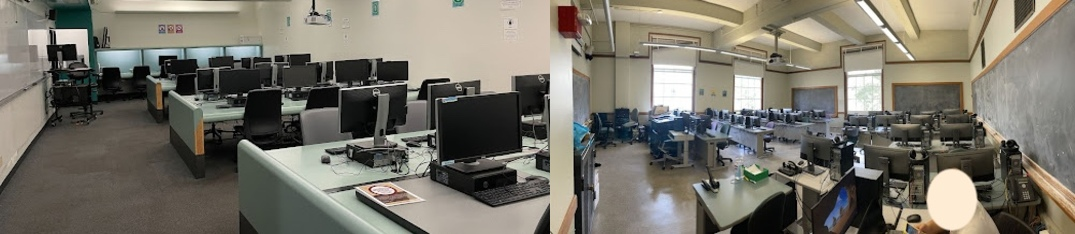
\includegraphics[width=\textwidth]{figs/labs}
  \caption{\label{fig:spaces}%
    In Fall 2023, we piloted
    computer-based testing for a 230-student course
    with part-time use of two shared computer labs, with operations funded by a
    research grant.  Since then we have used
    shared and dedicated spaces to scale up to $5,000+$ students in 24 courses
    from 16 departments, with
    a permanent and centrally-supported 100-seat facility opening in Fall 2026.
  }
\end{teaserfigure}

\begin{abstract}

As part of a larger research agenda focused on mastery learning,
we were inspired by the benefits of Computer-Based Testing Facilities (CBTFs)
reported by
the University of Illinois at Urbana-Champaign,
and in Fall 2023 we decided to pilot such a facility ourselves.
If successful, we intended to scale up and eventually serve
the whole campus, not just one or two CS courses. 
Three years later, our CBTF operation has grown to 20x 
(geometric mean of 120\% growth in seated exam-hours per semester), and serves
departments across campus.
Bootstrapping the initial effort led to important lessons---some
evident only with distant hindsight and the need to scale---from which we hope others
might benefit.
Our two main takeaways are as follows.
First, even in a small pilot, avoid adopting
processes that won't scale,
%% Exceptional situations should create $O(1)$ work per
%%   student or per instructor rather than $O(n)$ work for CBTF staff,
since student and faculty expectations are heavily influenced by the
  policies and procedures established during the pilot phase.
Second, while various campus units typically ``own'' lab facilities,
disabled-student proctoring,
instructional technology, room reservations, and so on, usually
  no one ``owns'' whole-course proctored exam administration.  You will have to create new
  administrative processes, disrupt existing ones, correct mistaken
  faculty assumptions, and coordinate across nonporous administrative
  boundaries.

\end{abstract}

\begin{comment}
  %% submitted abstract plain text:


As part of a research program on mastery learning, inspired by the benefits of Computer-Based Testing reported by the University of Illinois at Urbana-Champaign, in Fall 2023 we ran a pilot of such a facility ourselves. If the pilot succeeded, we intended to scale up and eventually serve the whole campus, not just one or two CS courses. Three years later, our CBTF operation is 20x larger and serving departments across campus; bootstrapping the initial effort led to important lessons---some evident only with long hindsight---from which we hope others might benefit. Our two main takeaways are as follows. First, even in a small pilot, avoid adopting processes that won't scale, since student and faculty expectations are heavily influenced by the initial policies and procedures. Second, while various campus units typically ``own'' lab facilities, proctoring for students with disabilities, instructional software and hardware maintenance, room reservations, and so on, usually no one "owns" whole-course proctored exam administration.  You will have to create new administrative processes, disrupt existing ones, correct mistaken faculty assumptions, and coordinate across nonporous administrative boundaries.


\end{comment}


%% keywords:
%% computer-based assessments, cs education, summative assessments

%% index terms:
%Social and professional topics > Professional topics > Computing
%education > Student assessment

\begin{CCSXML}
<ccs2012>
   <concept>
       <concept_id>10003456.10003457.10003527.10003540</concept_id>
       <concept_desc>Social and professional topics~Student assessment</concept_desc>
       <concept_significance>500</concept_significance>
       </concept>
 </ccs2012>
\end{CCSXML}

\ccsdesc[500]{Social and professional topics~Student assessment}


\maketitle



\section{Introduction}

Since before the COVID-19 pandemic, various CS and non-CS faculty at
our North American postsecondary higher-education
institution had been promoting mastery 
learning as a way of both improving 
pedagogy~\cite{Bloom68} and narrowing equity gaps~\cite{guskey2007closing}.
Since trustworthy and efficient summative assessment is an important
component of mastery learning,
we aimed to pilot a Computer-Based Testing
Facility (CBTF) modeled on the successful
experiences at
the University of Illinois at Urbana-Champaign~\cite{zilles-testing-less-trying} and
other institutions~\cite{downey-cbtf}.
Our goal was to
start with a single course and eventually spread the benefits of
mastery learning to all departments throughout the institution.
Because we believed that such a testing center should be a common good
and therefore centrally administered and resourced, scale-up would
require demonstrating the utility of the service beyond
engineering/STEM courses and departments,
centralizing its operations in a nonacademic campus unit,
and developing cross-unit funding and coordination models that did not
currently exist.

Our ``proto-CBTF'' pilot in Fall 2023 consisted of a single course with
230 students consuming about 1,000 student-exam-hours and proctored
largely by TAs and one-off student assistants.
2.5 years later, we have successfully scaled to 24 courses from 16 departments, enrolling over
5,000 undergraduates and accounting for over 45,000
seated exam-hours, proctored by a staff of 29 regular proctors (also student assistants).
These students take exams in one dedicated 30-seat CBTF and a second
shared 30-seat lab; the campus has since committed to opening a
dedicated 80--100 seat CBTF in Fall 2026 in a renovated building, 
and that new CBTF is already fully subscribed, months before opening.
All of this is now offered as  a ``common good'' campus service operated
by a comprehensive and
well-managed instructional technology unit, which also
has mature processes for hiring, onboarding, and supervision of
proctors (student assistants).
This paper describes the ``proto-CBTF'' bootstrap period with a few
details about the ``scale up'' period that led to the present moment.

The single course chosen for our pilot was an upper-division
software/systems course enrolling around 230 students.
During the COVID-19 pandemic, the course's quizzes had been converted
to the PrairieLearn assessment authoring
system\footnote{prairielearn.org} and were taken remotely using
videoconference-based proctoring.  Once the pandemic lockdown ended,
we decided to convert the 2.5-hour final exam (traditionally a written
final with a mix of short-answer and long-form questions) to be administered
in a prototype CBTF in Fall 2023.

A key property of the ``UIUC model'' we were trying to emulate
is that the exam incorporates enough randomness~\cite{chen-how-much-randomization} that its
integrity does not depend heavily on all
students take it simultaneously---a necessity since we had only about
57 seats in our proto-CBTF spaces, and a boon to students since they could
self-schedule their exam over a multi-day window.
The model also embodies other
practices that are important at scale but could  have been ignored for our single course;
since we planned to scale, we tried to avoid scale-thwarting
practices, indicating in the text
where we would have done things differently in hindsight.

We divide our experience into three categories: physical space and
configuration (Section~\ref{sec:physical}), IT infrastructure
(Section~\ref{sec:it}), and policies/coordination/communication (Section~\ref{sec:policy}).
Due to space constraints and our focus on operational lessons, we do
not discuss exam content.  In particular, we do not discuss the
process of moving from our paper-based exam to PrairieLearn, except to
state that we ended up with an exam that was in many ways as rich and
authentic as our paper-based final, and in some ways significantly
better.


\input{physical}
\input{it}
\input{ops}
\section{Funding, Process, and Policy}
\label{sec:policy}

\subsection{Messaging, or, Who Pays For All This?}

\lesson{Exam administration has many potential stakeholders. Each success attracts support; cast a wide
net to bootstrap flexible funding, and message your successes.} 

We began with an initial internal ``microgrant'' of US\$10,000 from the
Division of Undergraduate Education, based on presentations we had
made to multi-department audiences (e.g.\ Deans and Chairs) about the
benefits of mastery learning and the key role of computer-based
testing in supporting it.  This grant supported some initial work
to convert lower-stakes content to PrairieLearn, such as homeworks
and remote quizzes,
to demonstrate what would be
possible in a CBTF setting.
We then made every effort to spread the word about the benefits of mastery
learning, understanding that \emph{different supporters need to hear
different messages.\/}  Faculty are concerned about pedagogy but also
about the workload and quality-of-life of their TAs.  The SAC is
concerned about the overwhelming number of students needing proctoring
that accounts for exam accommodations.  Deans,
Chairs, and Vice-whatevers are concerned about how best to deploy
limited academic staff budgets to high-leverage activities, and most
agree that proctoring isn't one.
As PIs on the research grant, we got ourselves invited everywhere we could using every connection we
had: faculty lunches in our
own and colleagues' departments, college-level meetings of Deans and Chairs,
external industrial advisory board meetings, teaching and learning seminars.
Each time we gave a presentation, we tried to show incremental but
positive results that would resonate with that stakeholder.
Evangelizing everywhere, we believed, would help ensure that when
an opportunity appeared,  potential benefactors would be positively
predisposed to support the project.

While we have no counterfactual, we believe the approach worked:
after a few months we attracted additional
seed funding of US\$75,000 from the College of Engineering, in
recognition of the fact that the ``first wave'' of courses to
potentially benefit from the CBTF would be homed there.
Later, on the success of that funding, we won two expansive grants
totaling about US\$1.5M (shared with two 
other institutions) covering research and content development related
to mastery learning as well as CBTF operations.

Critically, all of these pools of money had considerable flexibility
in how they were spent, and there was some ``informal'' accounting
within the institution as well.  For example, we did not have to pay
to use the shared lab infrastructure since it was already a ``common
good'' service, and their staff were willing to put in some  modest
extra effort to help us run them as part-time CBTF spaces
without line-item financial compensation.
Similarly, we were able to borrow some internal IT staff time for various
aspects of on-site hosting and proctor hiring/supervision,
as well as having explicit support in the research grants for IT staff
time to manage and pay for
CBTF cloud resources.
As a result of these visible successes, when a large dedicated space miraculously became available as part of
a building remodel, central campus committed over US\$1.5M to convert
and operate it as a permanent CBTF starting in Fall 2026.

\subsection{Institutional Exam Policies}

\lesson{Consider asking forgiveness, rather than permission, for
accidentally transgressing the letter of the law in good faith.}

Many institutions have regulations related to when and/or where students can
take exams, especially final exams.
Our courses are classified as either having a
``written final exam'' or not, and that designation requires committee
approval to modify.
A course with a written final is assigned a specific, non-negotiable time and room
during finals week, student conflicts be damned.
Must a CBTF final overlap that time slot?
What if  \emph{all\/}  your students demand to take your final at that
time, and there aren't enough CBTF seats?
Does a computer-administered exam even count as a ``written final''?  How many
angels can dance on the head of a pin?

The CBTF paradigm is so thoroughly foreign
compared to ``traditional'' exam administration that you may have no
choice but to break a few eggs when faced with such conundra.
At our institution, strong student and faculty voices, positive or
negative, carry significant weight; hence our focus on
spreading the word, collecting positive testimonials, and
gathering and acting on negative feedback.
To date, students both with and without accommodations in two dozen
courses overwhelmingly
appreciate the scheduling flexibility, a majority  prefer CBTF exams
to paper exams, and no instructor who has tried CBTF exams
wants to go back. 

\label{sec:cheating}
A stakeholder we didn't expect to engage was our summer sessions program.
One student in the pilot performed much worse on the in-CBTF final than their  remote
quiz scores would predict;
investigation revealed that they had been systematically cheating on
the remote quizzes by having someone else take them and then
synthetically combining screencasts and live video to fool the remote
proctors.
This tactic was thwarted on the final by the CBTF's much higher exam
security.
That humbling and discouraging experience led us to 
adopt a CBTF-only policy for \emph{all\/} quizzes in the course---a change we were 
happy to make as instructors,
but which upset our summer sessions program since a course that cannot be
taken fully online has smaller revenue potential.


\section{Related Work}

Our 
work on scalable mastery learning ~\cite{Bloom68}, inspired by
Garcia et al.'s ``A's for All''~\cite{garcia-asforall} approach,
requires
the ability to administer frequent and
short summative
assessments that afford the
possibility of re-takes to demonstrate mastery on earlier
material~\cite{secondchanceexams}.
We believed that the extensive and
successful experience reported by the University of Illinois in
efficiently operating Computer-Based Testing
Facilities~\cite{zilles-testing-less-trying} was the most promising
approach to addressing that aspect of mastery learning.

Downey et al.~\cite{downey-cbtf} recently reported their experience
setting up a similar center at the University of California,
Riverside.
Our goals and experience are comparable to theirs, but whie they were
able to obtain full-time use of a secure room for their testing center
from the outset, we were limited to part-time use of existing
shared lab spaces.
In addition, their experience report was written after operating their
testing center for two academic quarters; the lessons reported here reflect two years of
hindsight and the experience of 20x scale-up, especially regarding
institution-wide concerns such as 
accessibility workflows, funding, and messaging/policy
issues.

Finally, mastery learning notwithstanding, many instructors who have
gravitated to our CBTF since the pilot were motivated 
by the need to secure assessments against unauthorized use
of AI.  In this context, the CBTF can be seen as the secure ``lane''
of the University of Sydney's ``two-lane approach to
assessment''~\cite{twolane}.

\section{Conclusion}

\lesson{Probably no unit at your institution ``owns'' exam
  administration: different pieces are owned by different units.}

Delivering exams securely and efficiently is not a simple function of
just the LMS, or just the firewall, or just the computer lab facilities, or just the
scheduling, or just the proctors; it requires coordination among all
these elements.
At most campuses, responsibility for any
one of them usually resides in a specific unit, but
nobody ``owns'' entire-course proctoring as a whole.
Achieving it requires new technical and social cooperation across
campus unit boundaries that are usually non-porous.   All of the
challenges we faced inherit from this challenge in some way.

Scaling up from our pilot has not been without additional challenges, including
getting the attention of the campus to recognize the value of
centrally funding a larger effort;
but it has led
to an assessment-delivery model that is (as others before us have found) 
\emph{far\/} superior to traditional exams in most respects.
The proof of the pudding is that the CBTF is now generating its own demand.

Our experience
demonstrates that the model pioneered at UIUC can be 
incrementally bootstrapped in an environment with different cultural
and administrative constraints without ``boiling the ocean.''  We are
confident that other institutions can do the same, and we
hope our lessons and reflections will help them do so.


\begin{acks}

The work described was supported by the College of
Engineering Dean's Office and  Office of the Vice Provost for Undergraduate
Education at UC~Berkeley, and California Education Learning Lab grants \#OPR19186 and \#00005919.
The project owes its success to
wide collaboration among faculty, College of Engineering staff, and Research,
Teaching \& Learning staff, including
Kevin Chan,
Shawna Dark,
James Fong,
Eric Fraser,
Jason Jung,
Dan Garcia
Jason Jung,
Tsu-Jae King Liu,
Catherine Koshland,
Greg Merritt,
Natalie Monta\~nez,
Erfan Moghadam,
Oliver O'Reilly,
Krystle Simon.

Thanks to Anastasia Kurda for proofreading and early feedback.
\end{acks}


\bibliographystyle{plain}
\balance
\bibliography{cbtf-bootstrapping}

\end{document}
\endinput
